\documentclass{article}
\usepackage[utf8]{inputenc}
\usepackage{float}
\usepackage{amsmath}
\usepackage{indentfirst}
\usepackage{amsfonts}
\usepackage{amssymb}
\usepackage{graphicx}
\usepackage{bm}
\usepackage{siunitx}
\usepackage [a4paper, left=3cm, right=3cm, top=2cm,bottom=3cm, heightrounded] {geometry}
\usepackage{multicol}
\usepackage{natbib}
\usepackage[english]{babel}
\usepackage{gensymb}
\usepackage[justification=centering]{caption}
\usepackage{ragged2e}
\usepackage{listings}
\usepackage{xcolor}
\usepackage{todonotes}
\usepackage{hyperref}
\usepackage[normalem]{ ulem }
\usepackage{soul}
\usepackage{subfig}
\usepackage{adjustbox} 
\usepackage[sorting=none]{biblatex} %Imports biblatex package
\addbibresource{references.bib}

\usepackage[utf8]{inputenc}
\usepackage[T1]{fontenc}

%New colors defined below
\definecolor{codegreen}{rgb}{0,0.6,0}
\definecolor{codegray}{rgb}{0.5,0.5,0.5}
\definecolor{codepurple}{rgb}{0.58,0,0.82}
\definecolor{backcolour}{rgb}{0.95,0.95,0.92}
%Code listing style named "mystyle"
\lstdefinestyle{mystyle}{
  backgroundcolor=\color{backcolour},   commentstyle=\color{codegreen},
  keywordstyle=\color{magenta},
  numberstyle=\tiny\color{codegray},
  stringstyle=\color{codepurple},
  basicstyle=\ttfamily\footnotesize,
  breakatwhitespace=false,
  breaklines=true,
  captionpos=b,
  keepspaces=true,
  numbers=left,
  numbersep=5pt,
  showspaces=false,
  showstringspaces=false,
  showtabs=false,
  tabsize=2
}
%"mystyle" code listing set
\lstset{style=mystyle}

%en tete+bas de page
\usepackage{fancyhdr}
\pagestyle{fancy}
\fancyhf{}
\fancyhead[L]{}
\fancyhead[C]{}
\fancyhead[R]{}

\fancyfoot[C]{\thepage}
\fancyfoot[L]{EPFL Center for Imaging}
\fancyfoot[R]{2025}
\renewcommand{\footrulewidth}{0.4pt}






%Page de titre

\begin{document}
\begin{titlepage}
\newcommand{\HRule}{\rule{\linewidth}{0.5mm}} % Defines a new command for the horizontal lines, change thickness here
\center % Center everything on the page

\includegraphics[width=0.7\linewidth]{epfl.png}\\[1cm] % Include a department/university logo - this will require the graphicx package
\textsc{\LARGE Ecole Polytechnique Fédérale de Lausanne}\\[2cm]
\HRule \\[0.4cm]
{ \huge \bfseries CSE Master Semester Project}\\[0.4cm] % Title of your document
\HRule \\[1.5cm]
\textsc{\LARGE Image reconstruction: CT denoising}\\[1cm]

\textsc{ 8 ECTS Semester project}\\[1cm]


\textsc{Gomes Almada Guillemin}\ Ismaël \\
\begin{figure}[H]
    \centering
    \includegraphics[scale=0.2]{Signatures.png}
    \label{fig:my_label}
\end{figure}

\textsc{ EPFL Center for Imaging}\\[1cm]
\textsc{Supervised by :}\\[0.2cm]
\textsc{Prof. Andò}\ Edward  \\ [0.1cm]
\textsc{Dr. Kashani}\ Sepand\\[0.1cm]
RX Solutions\ \\[1.2cm]


\textsc{\large Date :}\\[0.1cm]
\textsc{06 June 2025}\\

\end{titlepage}
%table des matières
\tableofcontents
\renewcommand{\contentsname}{Summary}
\thispagestyle{empty}
\newpage
\setcounter{page}{1}
%début texte
\section{Introduction}
Computed Tomography (CT) reconstruction is a non-destructive technique widely  used in imaging that enables the reconstruction of volumetric information about the internal structure of an object. By projecting X-rays through the object from various angles and recording their shadows, it is possible to determine the absorption profile of the material  and subsequently reconstruct the internal structure of the object. This process, known as image reconstruction, lies at the core of computational imaging. 
\medskip

\setlength{\parindent}{0pt}
Nowadays, however, the quality of reconstructed images is often compromised by noise and limited in data acquisition, which motivates the need for advanced denoising techniques. The aim of this project is to explore various potential techniques for enhancing CT image quality through denoising strategies, with a particular focus on scenarios involving the traditional filtered back projection method.

\section{Motivation}
In computational imaging, the X-ray transformation can be modeled as follows:
\begin{equation}
\mathbf{y} = R(\mathbf{x}) + \bm{\eta}
\end{equation}
where:


- \( \mathbf{x} \in \mathbb{R}^n \) the image to reconstruct,

- \( R \) the forward operator (i.e. X-ray transform (XRT)) ,

- \( \mathbf{y} \in \mathbb{R}^m \) the sinogram (i.e. the measured projections),

- \( \bm\eta \) the additive noise (typically Gaussian or Poisson).
\medskip

Once formulated this way, several methods can be employed to reconstruct the image \textbf{x}. Among them, Filtered Back Projection (FBP) is widely used in the scientific community due to its simplicity and computational efficiency \cite{karl_foundations_2023} \cite{koetzier_deep_2023}. This direct inversion method can be expressed as follows:

 \begin{equation}
\hat{\mathbf{x}}_{\mathrm{FBP}} = R^* (h(\mathbf{y}))
\end{equation}
With: 


- \( R^* \) the adjoint of the forward operator, 

- h a high/band pass filter,

- \( \mathbf{y} \) the sinogram (i.e. the measured projections),

- \( \hat{\mathbf{x}}_{\mathrm{FBP}}\) the reconstructed image

\medskip

It is important to note that using only the adjoint operator of $R$ is not sufficient for accurate reconstruction. The FBP formula is derived by inverting the Fourier Slice Theorem (FST).
One of the inversion steps is to apply the ramp filter, or an approximation thereof to mitigate noise effects, prior to back-projecting the sinogram into the image domain via $R^{*}$.\cite{tan_deep_2024}
\medskip

This method performs very well qualitatively and quantitatively under ideal conditions and is fast. However, it suffers from significant drawbacks:
\begin{itemize}
    \item It is highly sensitive to noise.
    \item It requires dense angular sampling for optimal results.
\end{itemize}

To illustrate these observations, the following experiment was conducted. Several sinograms of a concrete cross section were simulated using the forward operator, while varying the proportion of projections performed (i.e., the ratio of the total number of projections to 180). 

In addition, two Gaussian noise levels were introduced into the sinograms such that the resulting signal-to-noise ratios (SNR) were \textbf{35.9 [dB]} (representing a \textbf{low noise level}) and \textbf{25.9 [dB]} (representing a \textbf{high noise level}), relative to the corresponding noise-free sinogram. Afterward, the FBP algorithm was applied to the altered sinograms in order to reconstruct the internal structure of the object. 
\medskip

To begin with, we assess the performance of FBP under ideal conditions, that is, using a fully sampled and noise-free sinogram in following Figure \ref{fig:concrete+sino}.


\begin{figure}[H]%
    \centering
    \subfloat[]{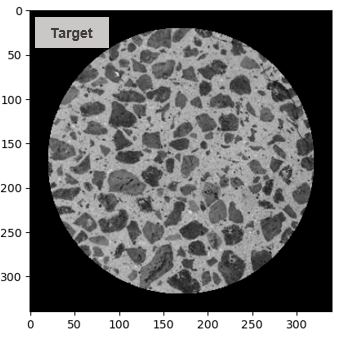
\includegraphics[width=5cm]{figures/concrete.png}\label{fig:concrete}}%
    \qquad
    \subfloat[]{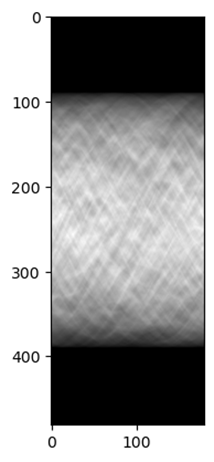
\includegraphics[width=2.5cm]{figures/sino.png}\label{fig:sino}}%
    \qquad
    \subfloat[]{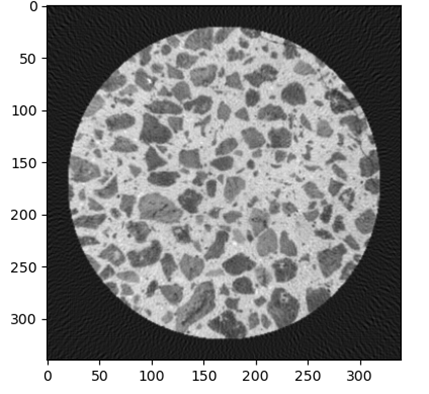
\includegraphics[width=5.35cm]{figures/fbp_100.png}\label{fig:fbp100}}%
    \caption{ \textbf{(a)} Cross-sectional image\footnotemark of a concrete sample, used as ground truth for CT reconstruction experiments. \textbf{(b)} Corresponding simulated sinogram using the forward operator with 100\% projection (i.e., one projection per degree) and no added noise. \textbf{(c)} Reconstruction using only FBP algorithm. }
    \label{fig:concrete+sino}
\end{figure}
\footnotetext{\url{https://ru.photo-ac.com/photo/29401522/concrete-surface-with-exposed-aggregate-cross-section}}

As shown in Figure\ref{fig:concrete+sino}, under ideal conditions, FBP performs very well. The reconstructed image exhibits good contrast, and the internal structure of the concrete is accurately recovered, even for very small details. However, one can observe the presence of high-frequency artifacts outside the object domain, which is a known characteristic of FBP. These artifacts are attributed to the high-pass filter (specifically the ramp filter) used within the FBP algorithm.
\medskip

However, outside the ideal case, FBP no longer performs as well, as illustrated in Figure \ref{fig:fbp_vary}.
\begin{figure}[H]
    \centering
    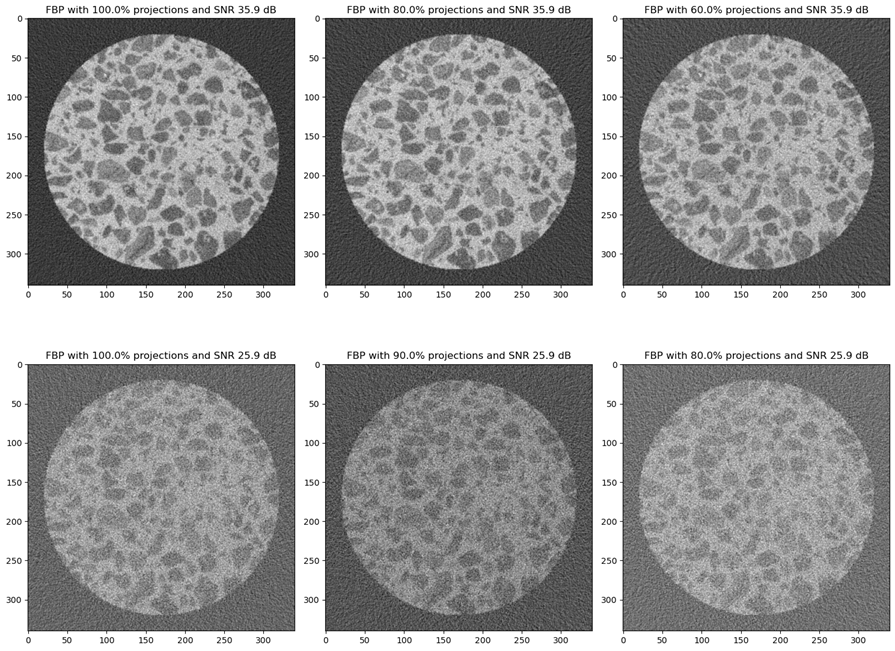
\includegraphics[scale=1]{figures/fbp_vary.png}
    \caption{Reconstructions obtained using the FBP algorithm under various proportions of projection and noise levels. \textbf{Top row:} Reconstruction from sinograms  with an SNR of 35.9 [dB] (low noise level)  and decreasing projection rates: 100\%, 80\%, and 60\%. \textbf{Bottom row:} Reconstruction from sinograms with an SNR of 25.9 [dB] (high noise level) and projection rates of 100\%, 90\%, and 80\%. }
    \label{fig:fbp_vary}
\end{figure}

Indeed, starting with the low noise scenario (top row of Figure \ref{fig:fbp_vary}), the reconstructed images are corrupted by noise. As the number of projections decreases, the image becomes less contrasted and more noisy. The reason is that the remaining noise in the sinogram (after ramp-filtering) is in the high frequencies, and these are backprojected into the image. For instance, in the case with 60\% of projections (reconstruction in the top right-hand corner), small features within the concrete structure are barely distinguishable, and the overall texture is degraded due to the noise. Additionally, the high-frequency artifacts observed around the image domain in the ideal case (Figure \ref{fig:fbp100}) are further amplified.
\medskip

In the case with a higher noise level (bottom row of Figure \ref{fig:fbp_vary}), the same degradation pattern is observed but to an even greater extent. In the reconstruction with 80\% of projections (reconstruction in the bottom right-hand corner), it becomes difficult to distinguish the foreground from the background within the concrete sample, and the texture is lost due to the overwhelming presence of noise.
\medskip

It is worth noting that, since the object domain is known, the peripheral artifacts could have been easily masked. However, no such post-processing was applied in order to objectively highlight the performance of the FBP algorithm alone.
\medskip

To conclude, these observations highlight the limitations of FBP when dealing with noisy and undersampled data. While the method remains effective under ideal conditions, its performance quickly deteriorates as noise increases or the number of projections decreases. To overcome these challenges and improve the quality of reconstructed images, several alternative strategies have been explored and are presented in following section. 



%These include pre-processing the sinograms, post-processing the reconstructed images, and model-based iterative reconstruction methods. Each of these approaches offers a different perspective on how to mitigate noise and artifacts in CT imaging.
 
\section{Experimental method}
This project investigates three different strategies to improve the quality of the reconstruction. These include:
\begin{itemize}
    \item Pre-processing the sinograms and apply FBP
    \item Post-processing the reconstructed images obtained from FBP
    \item Model-based iterative reconstruction methods with FBP as initialisation
\end{itemize}
 The idea is to still use the FBP method since it is fast and provides a physical sense of the reconstruction and from which improvements can be applied upstream or downstream. 
\subsection*{Pre-processing Approach}
As previously discussed, one of the main causes of quality degradation in FBP reconstructions is the presence of noise. Therefore, the idea here is not to modify the reconstruction algorithm itself, but rather to improve its input by denoising the sinogram before applying FBP. Signal processing (SP) or machine learning (ML) techniques can be employed at the data acquisition stage to suppress noise, thereby potentially limiting the propagation of artifacts during the reconstruction process.
\subsection*{Post-processing Approach}
The second approach focuses on improving the output of the FBP algorithm. The underlying idea is that modifying the raw data may distort the reconstruction process, and it might therefore be preferable to refine the output instead. As a result, the reconstruction pipeline remains unchanged, but an additional denoising step is introduced after FBP. This denoising can be carried out using either signal processing (SP) or machine learning (ML) methods.
\subsection*{Model-based Approach}
Finally, the third method can be seen as a more refined version of the post-processing approach. The idea here is to solve an optimization problem of the form (using the same notation as before):
$$
\hat{\mathbf{x}}_{\mathrm{opt}} = \arg\min_{\mathbf{x}} \left\| R(\mathbf{x}) - \mathbf{y} \right\|_2^2 + \lambda f(\mathbf{x})
$$
by using iterative methods, with the FBP image as the initial guess. This strategy leverages the fact that, with a reasonable starting point provided by FBP, only a few iterations may be needed to achieve a noticeable improvement.
\medskip

Moreover, this approach allows for the incorporation of a regularization term $f(\mathbf{x})$. The benefit of this term is to encode any knowledge we may have on \textbf{x}. This ranges from simple terms such as support constraints and positivity of the reconstructed image, as well as feature-enhancing terms such as Total Variation (TV) regularization. The latter promotes smooth surfaces with sharp edge transitions. Note that $\lambda$ is a parameter that can be tuned to control the strength of the regularization term.
\smallskip

Since several years, there has also been a push to incorporate ML methods into the model-based approach via Plug-and-Play (PnP) methods.
They consist in replacing classical $f(\mathbf{x})$'s with learned denoisers.

\section{Results and Discussion}
To assess the effectiveness of each approach, we focus on two representative scenarios previously shown to challenge the performance of FBP. Specifically, we consider two cases: 
\begin{itemize}
    \item Sinogram with 60\% projections and low noise
    \item Sinogram with 80\% projections and high noise
\end{itemize}
  These configurations are used as benchmarks to evaluate whether the proposed approaches can outperform FBP by comparing their performance in terms of noise suppression, detail preservation, contrast, artifact reduction and computation time. 
\subsection{Qualitative analysis}

\subsubsection*{Pre-processing Approach}
The results obtained using pre-processing methods with SP or ML approach for sinogram denoising before applying FBP algorithm are presented in \ref{fig:pre_pro}.

The first column corresponds to the reconstructions obtained using the standard FBP algorithm without any pre-processing.


In the second column, a pre-filtering step is applied using the ramp-cosine filter (SP approach). This filter is simply a cosine function multiplied by the ramp filter. It preserves the ability to suppress low-frequency components, while also slightly attenuating high-frequency components that could come from noise.

Finally, the third column shows the results obtained by denoising the sinogram with a neural network called "MAXIM"\footnote{\url{https://github.com/google-research/maxim}}, followed by FBP reconstruction (ML approach). MAXIM is a pretrained multi-axis MLP neural network developed by Google \cite{tu_maxim_2022}. This model was chosen because it is implemented in JAX\footnote{\url{https://docs.jax.dev/en/latest/quickstart.html}}, which allows for accelerated computation through Just-In-Time (JIT) compilation. Furthermore, we chose an existing model (MAXIM) since our goal was not to conduct research on a specific NN architecture in this project.
Rather, we sought to investigate whether ML can be incorporated in the reconstruction pipeline to enhance FBP outputs. This is why we went with a pre-existing architecture.

\begin{figure}[H]
    \centering
    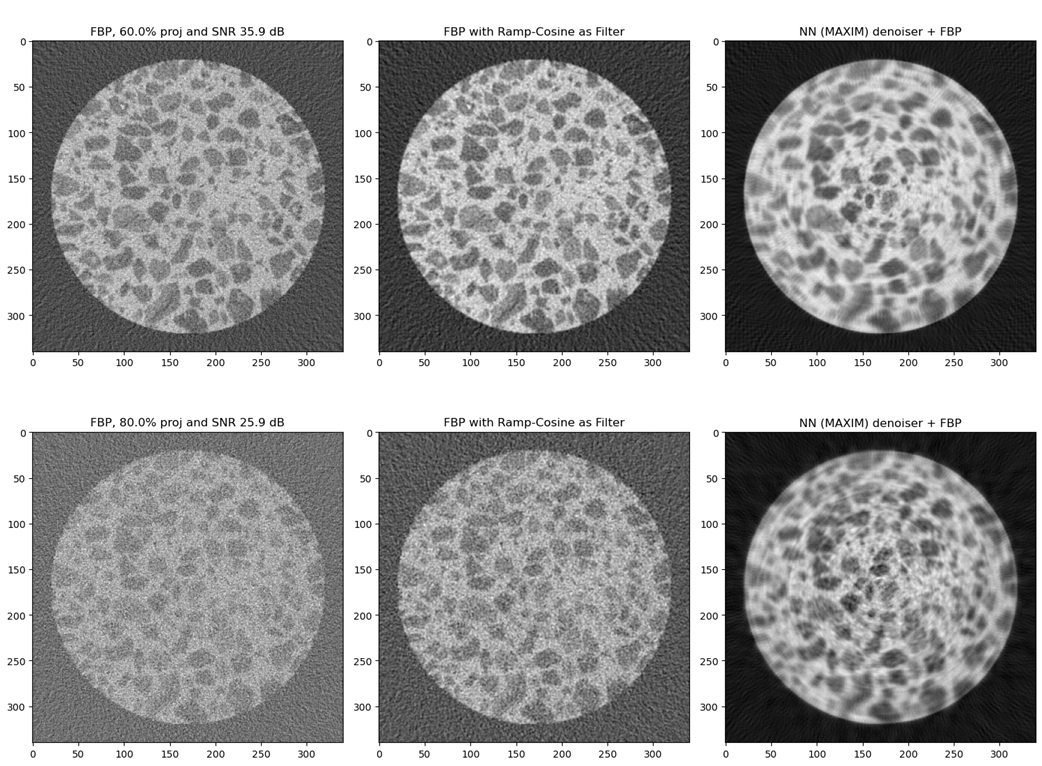
\includegraphics[scale=0.85]{figures/pre_pro.png}
    \caption{ Comparison of FBP reconstructions using different sinogram pre-processing methods in the case with 60\% projections and low noise level (\textbf{Top}) and the case with 80\% projections and high noise level (\textbf{Bottom}).
\textbf{Left:} Standard FBP reconstructions without any pre-processing.
\textbf{Center:} FBP reconstructions after denoising the sinograms using a ramp-cosine filter.
\textbf{Right:} Reconstructions after denoising the sinograms using the pretrained MAXIM neural network, followed by FBP}
    \label{fig:pre_pro}
\end{figure}
In the case of the signal processing method (middle column Figure \ref{fig:pre_pro}), the resulting image shows a slight improvement compared to the standard FBP reconstruction. While the overall contrast is marginally enhanced, noise remains clearly visible in both cases (high and low level noise), and the high-frequency artifacts surrounding the object are still present.
\medskip

In contrast, the machine learning-based approach (right column Figure \ref{fig:pre_pro}) significantly reduces these peripheral artifacts and improves the image contrast. However, one can also observe the emergence of some hallucinated/blurry structures, particularly near the circular boundary of the concrete sample, which suggests that the model introduces non-physical details in certain regions. This phenomenon is explained by the nature of the denoising NN. Indeed, MAXIM is designed for natural 2D image denoising. Since sinograms are fundamentally 1D signals arranged across projection angles, applying such a neural network to this type of data distorts the 1D signals by performing cross-projection operations. As a result, the raw sinogram is altered in a way that introduces non-physical features into the reconstruction. 

In general, the issue with pre-trained models is that they exist mostly for 2D/3D images and not 1D signals. As a consequence, when applied to 1D sinograms, we obtain hallucinated/blurry structures in the reconstructed images. Despite these limitations, the results remain encouraging. This suggests that it would be worth investigating this approach further by training a dedicated machine learning model specifically designed to denoise 1D sinograms.

\subsubsection*{Post-processing Approach}
We now evaluate in Figure \ref{fig:post_pro} the post-processing approach, where denoising is applied directly to the output of the FBP reconstruction.

As in previous Figure \ref{fig:pre_pro}, the left column corresponds to the baseline case using only the FBP algorithm without any denoising.

In the middle column, a simple signal processing technique, median filter, was applied to the FBP output.

In the right column, the same neural network (MAXIM) as in the pre-processing approach was used, but this time applied to the reconstructed image provided by FBP rather than the sinogram.

\begin{figure}[H]
    \centering
    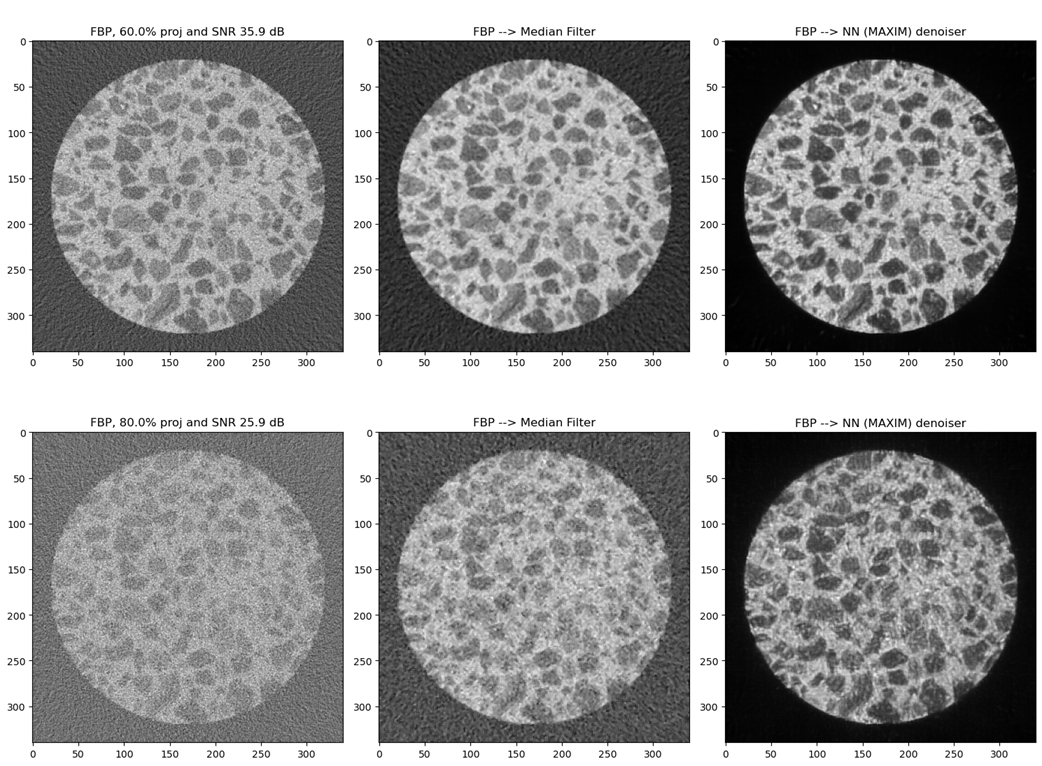
\includegraphics[scale=0.85]{figures/post_pro.png}
    \caption{Comparison of image reconstructions after post-processing FBP output in the case with 60\% projections and low noise level (\textbf{Top}) and the case with 80\% projections and high noise level (\textbf{Bottom}).
\textbf{Left:} Standard FBP reconstructions without any post-processing.
\textbf{Center:} Results after applying a median filter directly to the FBP outputs.
\textbf{Right:} Results after applying the pretrained MAXIM neural network to the FBP reconstructions.}
    \label{fig:post_pro}
\end{figure}

As observed previously, the signal processing approach (middle column Figure \ref{fig:post_pro}) does not lead to a significant improvement in image quality compared to the baseline FBP method. The median filter does reduce noise and improve contrast with respect to only using FBP algorithm, but the result remains sub-optimal, especially in the high noise case. Furthermore, we still have high-frequency artifacts that persist around the sample boundaries.
\medskip

In contrast, the machine learning approach (right column Figure \ref{fig:post_pro}) produces a more noticeable improvement. The noise is substantially reduced and the contrast is close to the ground truth image (Figure \ref{fig:concrete}). Interestingly,  even though the ML model has no knowledge that the image background should be zero outside the central circle, it does decide to remove the artifacts. 

However, when examining the bottom-right image (80\% projections, high noise level), one can observe that the denoising operation appears to introduce artificial textures that are not present in the ground truth image. In the absence of a reference, these hallucinated features could easily be mistaken for real image textures, which raises concerns about the interpretability and reliability of the denoising by employing a ML method.


\subsubsection*{Model-based Approach}
Finally, we turn to the model-based approach in Figure \ref{fig:model_based}. As before, the left column shows the reconstruction obtained using only the FBP algorithm.

In the middle column, we present the reconstruction obtained by solving the following constrained optimization problem:

\begin{equation}
\hat{\mathbf{x}}_{\mathrm{opt}} = \arg\min_{\mathbf{x} \in \mathcal{C}} \left\{ \left\| R(\mathbf{x}) - \mathbf{y} \right\|_2^2 + \lambda \left\| \nabla \mathbf{x} \right\|_1 \right\}
\end{equation}
where $\mathcal{C}$ encodes both the support constraint and the positivity constraint, and $\left\| \nabla \mathbf{x} \right\|_1$  denotes the Total Variation (TV) regularization term. This formulation aims to suppress noise by smoothing the reconstruction with TV regularization while enforcing physical priors on the reconstruction domain. The problem was solved using a proximal gradient descent algorithm, which is well-suited for handling non-smooth regularization terms and constraint sets. 360 iterations were performed in both low and high noise level cases, using a step size $\alpha = 10^{-5}$, a regularization weight $\lambda = 10^{-1}$ and the FBP reconstructions were used as the initial guess.
\medskip

In the right column, we investigate a Plug-and-Play (PnP) variant of the model-based approach. Unlike in previous sections, we do not use MAXIM here, as it was shown to introduce hallucinated patterns. Instead, we use a learned non-convex regularizer developed by the Bioimaging Group at EPFL. The optimization problem can be formulated as follows:
\begin{equation}
\hat{\mathbf{x}}_{\mathrm{opt}} = \arg\min_{\mathbf{x}} \left\{ \left\| R(\mathbf{x}) - \mathbf{y} \right\|_2^2 + \lambda Reg_{CNC}(\mathbf{x}) \right\}
\label{eq:CNC_fini}
\end{equation}
where $Reg_{CNC}(\mathbf{x})$ represents the learned regularization term. This neural network was specifically designed to avoid hallucinations and offers competitive denoising performance while relying on fewer than 15,000 parameters \cite{goujon_learning_2024}.

A PyTorch (PT) implementation of the model\footnote{\url{https://github.com/axgoujon/weakly_convex_ridge_regularizer/tree/main}} is available from the original paper, along with a pre-trained model trained on the BSD500 dataset \cite{arbelaez_contour_2011}. The PT version is somewhat rigid and makes it difficult to modify internal components. This limited our ability to retrain the model on our own synthetic dataset, which was specifically designed to mimic the structure of the concrete sample with varying geometric shapes, textures, and noise levels. For this reason, we attempted to port the model to JAX in order to experiment the model more freely and take advantage of JAX’s features. However, a literal translation of the PT model to JAX turned out to be difficult and took a significant portion of the semester. Unfortunately, the conversion could not be completed in time. As a fallback, we used the pre-trained PT model to produce qualitative results presented in the right column of Figure \ref{fig:model_based} with 47 and 64 iterations in low and high noise cases respectively. These give an idea of how the method performs in practice, but the reported timing results should be taken with a grain of salt.
\medskip

Note that in order to use the pretrained PT implementation of the $Reg_{CNC}$ regularizer, the initial guess must be normalized. Therefore, the FBP reconstructions were normalized before being passed as input.
\smallskip

Moreover, in addition to the parameter $\lambda$, the regularizer $Reg_{CNC}$ also requires specifying the standard deviation of the noise. Indeed, to use the PT implementation of $Reg_{CNC}$, the standard deviation of the noise must be provided as input. In our case, since the noise was deliberately added and the ground truth is available, this value could be easily estimated. However, in a real-world setting, estimating the noise level is more challenging. One simple approach would be to select a region in the image that contains only background noise (e.g., outside the sample boundary in our case) and compute the standard deviation. Nevertheless, this method assumes spatially uniform noise and may therefore be unreliable. A more accurate alternative would be to perform a calibration procedure using a known reference image. By computing its sinogram and reconstructing it under realistic conditions, one could estimate the noise by subtracting the ground truth from the reconstructed image, and subsequently determine its standard deviation.


\begin{figure}[H]
    \centering
    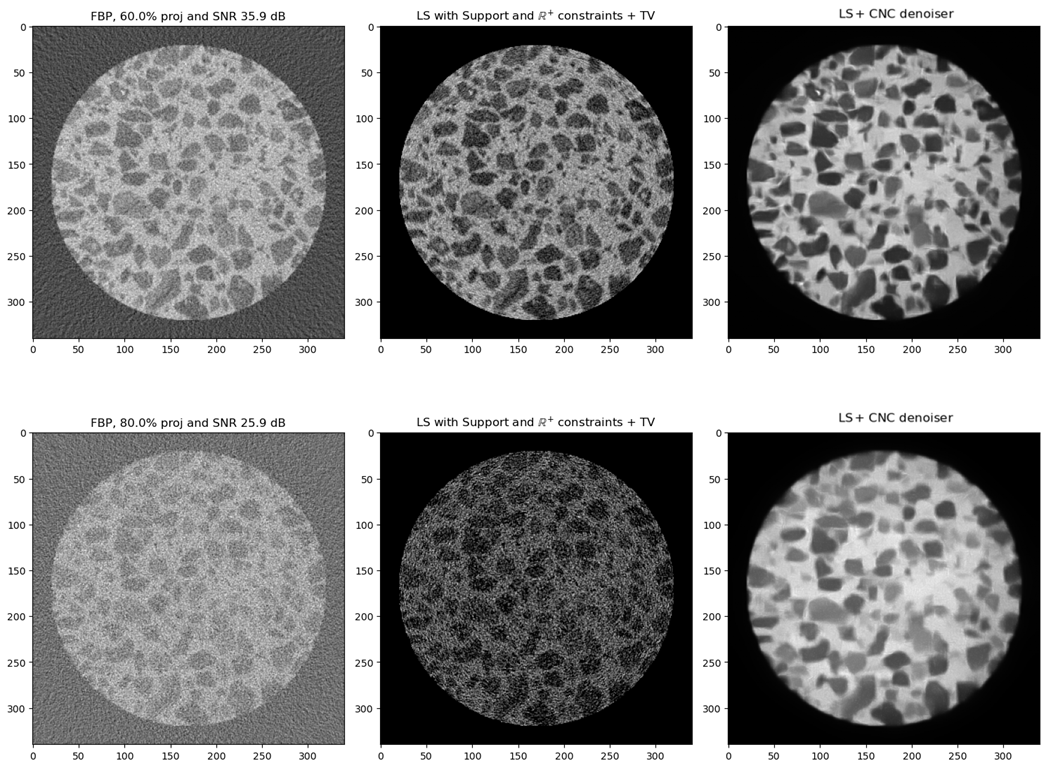
\includegraphics[scale=0.83]{figures/image.png}
    \caption{Comparison of model-based reconstruction approaches in the case with 60\% projections and low noise level (\textbf{Top}) and the case with 80\% projections and high noise level (\textbf{Bottom}).
\textbf{Left:} Standard FBP reconstructions without any other processing step.
\textbf{Center:} Results of solving a constrained least squares problem with support and positivity constraints and TV regularization.
\textbf{Right:} Results of same  least squares problem, but by using a pre-learned non-convex regularizer instead.}
    \label{fig:model_based}
\end{figure}
One can see in Figure \ref{fig:model_based} that both methods (SP and ML) perform better than the simple FBP reconstruction in terms of noise reduction and contrast.
\medskip

 When examining the middle column (SP method), we observe that the artifacts around the main object have been removed thanks to the support constraint. Moreover, for the low noise case (top), the reconstructed image exhibits intensities and contrast that are much closer to the ground truth presented in Figure \ref{fig:concrete}.
However, in terms of denoising performance and contrast, there are still noticeable limitations in the case of high noise level. 
\medskip

For the ML-based model (right column), an overall improvement in image quality is observed: The artifacts around the object boundary have been effectively removed. The contrast is visually comparable to the ground truth (Figure \ref{fig:concrete}) in both low and high noise scenarios. Additionally, the noise is no longer perceptible.
\medskip

However, the CNC regularizer appears to have removed all texture from the images. Our hypothesis is that the noise present in FBP reconstructions is no longer i.i.d across pixels, although it remains Gaussian. Although the initial noise added to the sinogram was i.i.d Gaussian, the FBP reconstruction process propagates the noise without preserving the i.i.d property. This may explain why the CNC regularizer, which was specifically trained on i.i.d Gaussian noise, fails to preserve the texture while denoising.

Furthermore, as said before,  the pretrained CNC denoiser used here was trained on natural images from the BSD500 dataset, not on CT-specific data. This mismatch may also contribute to the observed oversmoothing effect.


\subsection{Quantitative analysis}
We now turn to the quantitative analysis of the different methods. Three metrics are used to evaluate performance: the contrast-to-noise ratio (CNR), the signal-to-noise ratio (SNR), and the computation time, which provides insight into the computational cost of each method.
\medskip

The CNR is defined as the difference between the average signal in a region of interest ($\mu_{\mathrm{signal}}$) and the average background value $(\mu_{\mathrm{background}})$, divided by the standard deviation of the noise ($\sigma_{\mathrm{noise}}$) \cite{brian_x-ray_2020}:
\begin{equation}
\mathrm{CNR} = \frac{|\mu_{\mathrm{signal}} - \mu_{\mathrm{background}}|}{\sigma_{\mathrm{noise}}}
\end{equation}
A higher CNR indicates better contrast in the reconstructed image. In our experiments, the CNR was computed over three distinct regions of interest (see Figure \ref{fig:CNR_area}), and the average of these values was used to facilitate comparison across methods.

Regarding computation time, all experiments were performed on a CPU (AMD Ryzen 7 7840HS). For detailed information about the software libraries and their respective versions, please refer to the project’s GitHub repository \footnote{\url{https://github.com/igomes1/Deep-denoising-X-ray-CT-reconstruction/tree/main}}.



\begin{table}[H]
\centering
\begin{adjustbox}{width=1\textwidth}

\begin{tabular}{cc|cc|cc|cc|}
\cline{3-8}
                                                                                                   &                             & \multicolumn{2}{c|}{\textbf{Pre-processing}}                     & \multicolumn{2}{c|}{\textbf{Post-processing}}                    & \multicolumn{2}{c|}{\textbf{Model based}}         \\ \cline{2-8} 
\multicolumn{1}{c|}{\textbf{}}                                                                     & \textbf{FBP}                & \multicolumn{1}{c|}{\textbf{SP}}                 & \textbf{ML}   & \multicolumn{1}{c|}{\textbf{SP}}                 & \textbf{ML}   & \multicolumn{1}{c|}{\textbf{SP}}  & \textbf{ML}   \\ \hline
\multicolumn{1}{|c|}{\textbf{Mean CNR {[}-{]}}}                                                    & 2.47 / 0.95                 & \multicolumn{1}{c|}{4.68 / 1.79}                 & 9.59 / 5.65   & \multicolumn{1}{c|}{6.43 / 2.28}                 & 6.66 / 3.81   & \multicolumn{1}{c|}{2.88 / 0.93}  & 22.03 / 21.07 \\ \hline
\multicolumn{1}{|c|}{\textbf{SNR {[}dB{]}}}                                                        & 11.82 / 5.39                & \multicolumn{1}{c|}{14.58 / 9.30}                & 11.36 / 13.13 & \multicolumn{1}{c|}{15.10 / 11.18}               & 14.13 / 13.56 & \multicolumn{1}{c|}{13.60 / 5.25} & 14.53 / 10.80 \\ \hline
\multicolumn{1}{|c|}{\textbf{\begin{tabular}[c]{@{}c@{}}Computation \\ time {[}s{]}\end{tabular}}} & \textless{}1 / \textless{}1 & \multicolumn{1}{c|}{\textless{}1 / \textless{}1} & 9 / 13        & \multicolumn{1}{c|}{\textless{}1 / \textless{}1} & 16 / 16       & \multicolumn{1}{c|}{253 / 331}    & \textless{}5 / \textless{}5         \\ \hline
\multicolumn{1}{|c|}{\textbf{JIT}}                                                                 & No                          & \multicolumn{1}{c|}{No}                          & No            & \multicolumn{1}{c|}{No}                          & No            & \multicolumn{1}{c|}{Yes}          & No         \\ \hline
\end{tabular}
\end{adjustbox}
\caption{Quantitative comparison of the reconstruction methods across three criteria: CNR, SNR, and computation time. Results are reported for both low noise (left value) and high noise (right value) sinograms. "JIT" indicates whether Just-In-Time compilation was used.}

\label{tab:quant}

\end{table}
Overall, the quantitative results in Table \ref{tab:quant} are consistent with the qualitative observations discussed above. Across all reconstruction strategies, both CNR and SNR metrics improve compared to using the FBP algorithm alone. The only exception is the model-based approach using signal processing, which struggles to improve image quality in terms of both CNR and SNR in the high noise scenario, as previously observed in the qualitative analysis.
\medskip

With respect to Table \ref{tab:quant}, the machine learning approaches demonstrate superior performance compared to traditional signal processing methods in terms of CNR (at least for the regions of interest considered). In particular, the ML-based model reconstruction clearly outperforms all other methods, achieving the highest CNR values and confirming its strong capability in enhancing image contrast.
\medskip

Regarding noise (SNR), when each method category (pre-processing, post-processing, and model-based) is considered separately, signal processing  approaches tend to perform better in the low noise configuration than machine learning approaches. However, they become limited and are outperformed by machine learning approaches in the high noise scenario.


It is worth noting that the highest SNR is achieved by the post-processing SP method, although the model based with ML closely follows. This result may seem surprising, given that the model based ML reconstruction appeared to eliminate noise entirely in the visual analysis. However, the CNC regularizer also removed much of the image’s texture by over-smoothing it, which negatively impacts the SNR metric, since SNR is computed through direct pixel-wise comparison between the reconstruction and the ground truth.
\medskip

In terms of computation time, SP methods in the pre- and post-processing pipelines are nearly instantaneous on CPU (<1 [s]), similar to the FBP baseline. In contrast, ML methods require significantly more time, largely due to the computational complexity of the neural networks. Model-based methods with SP approach is by far the most time consuming, reflecting the cost of iterative optimization with 360 iterations. It is worth noting that the model-based approach using the CNC regularizer takes less than 5 seconds to run, which is a reasonable computation time. This efficiency is due to the relatively small number of iterations required, as well as the simple architecture of the model, which contains fewer than 15,000 parameters. 
\bigskip

In summary, both qualitative and quantitative analyses demonstrate that all proposed approaches improve the baseline FBP reconstruction in terms of noise reduction and contrast enhancement. Traditional signal processing methods perform well for noise suppression in low noise scenarios, but are outperformed by machine learning approaches when the noise level increases. In terms of contrast, ML-based methods consistently yield better results across all configurations, but care must be taken due to possible hallucinations by employing this kind of method. 


Among all tested methods, the model-based approach using the CNC regularizer stands out as the most balanced solution. It achieves a contrast level close to that of the ground truth and an SNR comparable to the best value obtained in this study with a reasonable computation time. Furthermore, it is worth noting that the SNR of this method can be further improved by retraining $Reg_{CNC}$ on a dataset specifically tailored for CT-reconstruction.

\section{Conclusion}
To conclude, the motivation behind this project was to address the limitations of the Filtered Back Projection algorithm in computed tomography image reconstruction, particularly under noisy and undersampled acquisition conditions. Although FBP is widely used due to its speed, quality and simplicity, it is highly sensitive to noise and produces artifacts, especially when the number of projections is reduced or when the data is corrupted by noise.
\medskip

To improve the reconstruction quality while preserving the advantages of FBP, three families of strategies were explored: (i) \textbf{Pre-processing the input of FBP}, (ii) \textbf{Post-processing the output FBP} and (iii) \textbf{Model based approaches with FBP output as initial guess}.
Each category was implemented using both classical signal processing techniques and more recent machine learning methods. 
\medskip

Both qualitative and quantitative analyses showed that all approaches provide improvements over standard FBP in terms of noise suppression and contrast enhancement. Signal processing methods proved effective in low noise settings, particularly for SNR, but were consistently outperformed by ML approaches when the noise level increased. ML methods yielded significantly better contrast, as reflected in higher CNR values.
\medskip

Among all tested methods, the model-based approach with the CNC regularizer offered the best overall performance. It combined a contrast level close to that of the ground truth with an SNR that rivaled the best results of classical methods, all while maintaining a reasonable computation time.
\medskip

As a next step, it would be valuable to retrain the CNC regularizer on a CT-specific dataset in order to further improve its performance. Additionally, although the ML-based pre-processing approach was shown to introduce hallucinations, due to the use of a denoiser originally designed for 2D natural images, the overall reconstruction quality remained relatively good. This observation opens up an interesting direction: designing a dedicated machine learning model specifically tailored to denoise 1D sinogram signals. Such a model could potentially yield improved performance, but care must be taken with respect to the interpretability of the results. 






\newpage
\section{Appendix}
\begin{figure}[H]
    \centering
    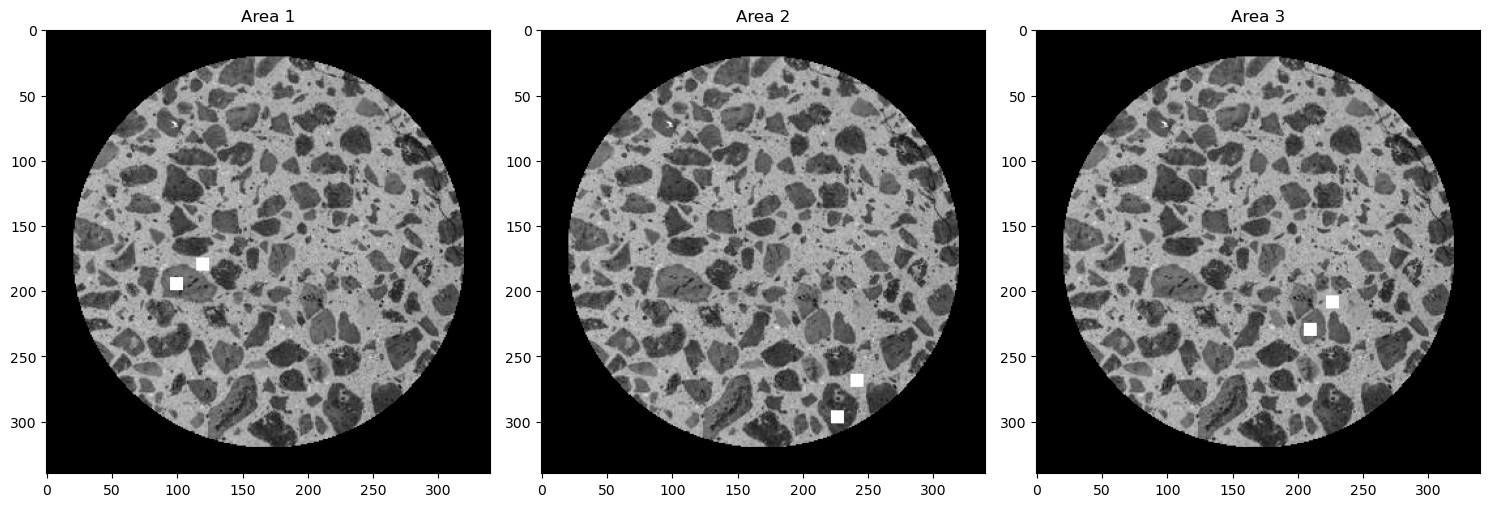
\includegraphics[scale=0.3]{figures/CNR_area.png}
    \caption{Visualization of the three regions of interest (ROI) used for computing the contrast-to-noise ratio (CNR). Each image highlights one ROI, with the signal and background areas indicated by white squares. The mean CNR reported in Table \ref{tab:quant} corresponds to the average value computed over these three regions.}
    \label{fig:CNR_area}
\end{figure}
\newpage
\printbibliography
Artificial Intelligence tools were used to assist in translating and reformulating the text of this report. They also contributed to the writing of figure and table captions and also introduction and conclusion sections.
\end{document}

